%! Author = Omar Iskandarani
%! Title = Time Dilation in a 3D Superfluid Æther Model, Based on Vortex Core Rotation and Ætheric Flow
%! Date = May 23, 2025
%! Affiliation = Independent Researcher, Groningen, The Netherlands
%! License = CC-BY 4.0
%! ORCID = 0009-0006-1686-3961
%! DOI = 10.5281/zenodo.15566319



\documentclass[a4paper,12pt]{article}

% Page Geometry
\usepackage[a4paper, margin=2cm]{geometry}

% Language, Encoding, Fonts
\usepackage[utf8]{inputenc}
\usepackage[T1]{fontenc}
\usepackage{lmodern}
\usepackage[english]{babel}

% Colors, Graphics, Diagrams
\usepackage{graphicx}
\usepackage{tikz}
\usetikzlibrary{arrows.meta, positioning}
\usepackage{pgfplots}
\pgfplotsset{compat=1.18}
\usepackage{xcolor}

% Math and Physics
\usepackage{amsmath, amssymb, physics}
\usepackage{siunitx}

% Tables and Figures
\usepackage{float}
\usepackage{booktabs}
\usepackage{array, tabularx, makecell, multirow}
\renewcommand{\arraystretch}{1.5}
\renewcommand{\floatpagefraction}{.8}
\usepackage[font=footnotesize]{caption}
\usepackage{subcaption}

% Code and Listings
\usepackage{listings}
\lstset{basicstyle=\ttfamily\footnotesize, breaklines=true}

% TOC Customization
\usepackage{tocloft}
\setcounter{tocdepth}{4}
\renewcommand{\cftsecfont}{\bfseries}
\renewcommand{\cftsubsecfont}{\itshape}
\renewcommand{\cftsecleader}{\cftdotfill{5}}
\renewcommand{\contentsname}{\centering \Huge\textbf{Contents}}

% Links and Metadata
\usepackage{hyperref}
\hypersetup{
    colorlinks=true,
    linkcolor=blue,
    citecolor=blue,
    urlcolor=blue,
    pdftitle={The Vortex Æther Model},
    pdfauthor={Omar Iskandarani},
    pdfkeywords={vorticity, gravity, æther, fluid dynamics, time dilation, VAM}
}
\usepackage{bookmark} % PDF bookmarks

% Bibliography
\usepackage[numbers]{natbib} % Or switch to biblatex if preferred

% Line and Hyphenation
\usepackage[none]{hyphenat}
\usepackage{amsfonts}


\sloppy

\begin{document}

\title{Time Dilation in a 3D Superfluid Æther Model, Based on Vortex Core Rotation and Ætheric Flow}
    \date{\today}
    \author{
        Omar Iskandarani\\
        \small Independent Researcher, Groningen, The Netherlands
        \thanks{\texttt{info@omariskandarani.com}}
        \thanks{ORCID: \href{https://orcid.org/0009-0006-1686-3961}{0009-0006-1686-3961} \quad DOI: \href{https://doi.org/10.5281/zenodo.15566319}{10.5281/zenodo.15566319} \quad License: \href{https://creativecommons.org/licenses/by/4.0/}{CC-BY 4.0}}
        \noindent\thanks{\textbf{Keywords:} \textit{time dilation, superfluid æther, Vortex Æther Model, vortex dynamics, emergent time, fluid spacetime, special relativity, Lorentz factor, analog gravity, 3D vortex structures, quantized circulation, relativistic effects, topological matter, fluid mechanics, vortex clock}}
    }
    \maketitle

\section*{Abstract}
In this paper we derive time dilation equations within a 3D Euclidean superfluid-like æther model. In the Vortex-Æther Model (VAM) we consider a \textit{vortex} as a topologically conserved rotation field in a superfluid-like medium. In this framework, fundamental particles are modeled as vortex nodes and time is defined by the intrinsic angular rotation of their vortex cores. The goal is to replace the spacetime curvature concept of general relativity (GR) with quantized angular velocity fields in a flat-space æther, while reproducing all experimental predictions of time dilation under GR and special relativity (SR). We provide first-principles derivations, grounded in fluid dynamics and vortex mechanics, and express the time dilation factors in terms of fundamental constants such as the Planck time and maximum force. The different modes of motion of a vortex are shown schematically in Figure~\ref{fig:rotation-translation}.

\begin{figure}[H]
        \centering
        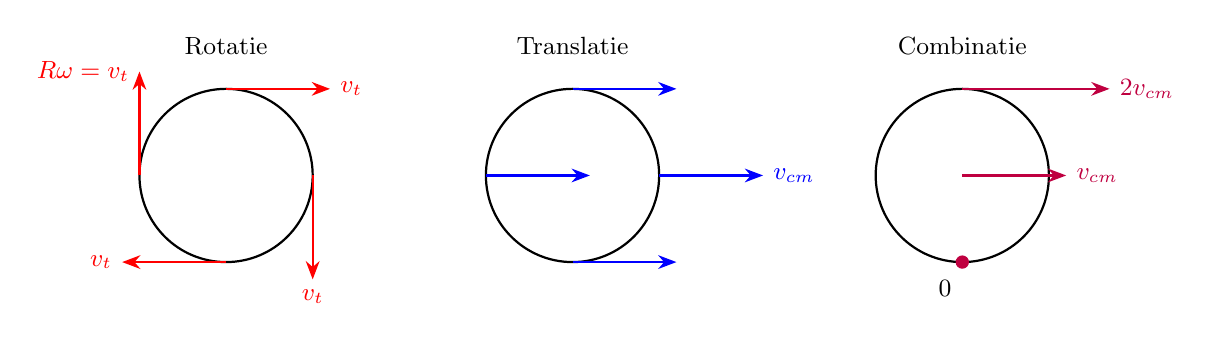
\begin{tikzpicture}[scale=1.1, >=Stealth, every node/.style={font=\small}]
            % First: Pure Rotation
                \node at (-3,2.5) {Rotatie};
                \draw[thick] (-3,1) circle (1);
                \draw[->, red, thick] (-4,1) -- (-4,2.2) node[left] {$R\omega = v_t$};
                \draw[->, red, thick] (-3,2) -- (-1.8,2) node[right] {$v_t$};
                \draw[->, red, thick] (-3,0) -- (-4.2,0) node[left] {$v_t$};
                \draw[->, red, thick] (-2,1) -- (-2,-0.2) node[below] {$v_t$};

            % Second: Pure Translation
                \node at (1,2.5) {Translatie};
                \draw[thick] (1,1) circle (1);
                \draw[->, blue, thick] (0,1) -- (1.2,1);
                \draw[->, blue, thick] (2,1) -- (3.2,1) node[right] {$v_{cm}$};
                \draw[->, blue, thick] (1,0) -- (2.2,0);
                \draw[->, blue, thick] (1,2) -- (2.2,2);

            % Third: Combined Motion
                \node at (5.5,2.5) {Combinatie};
                \draw[thick] (5.5,1) circle (1);
                \draw[->, thick, purple] (5.5,2) -- (7.2,2) node[right] {$2v_{cm}$};
                \draw[->, thick, purple] (5.5,1) -- (6.7,1) node[right] {$v_{cm}$};
                \filldraw[purple] (5.5,0) circle (2pt);
                \node at (5.3,-0.3) {$0$};
        \end{tikzpicture}
        \caption{Schematic representation of three modes of motion of a vortex in the æther model. \textbf{(Left)} Pure rotation with local tangential velocity $v_t = R\omega$. \textbf{(Middle)} Translation with velocity $v_\text{cm}$ without internal rotation. \textbf{(Right)} Combining both leads to a relative velocity that differs over the vortex circumference: $v_\text{rel} = v_t + v_\text{cm}$.}
        \label{fig:rotation-translation}
\end{figure}

\begin{figure}[htbp]
    \centering
    \includegraphics[width=0.85\textwidth]{02_cylinder_flow}
    \caption{Visualization of flow around a fixed cylinder as an analogy for æther flow around a stable vortex in the æther model. The uniform background flow is locally distorted by the presence of the vortex structure. This classical potential flow profile forms the basis for later interpretations of æther interactions in the model.}
    \label{fig:cylinderflow}
\end{figure}

\section{Introduction}
In a modern revival of Lord Kelvin's vortex-atom hypothesis of 1867~\cite{Kelvin1867-vortex}, we consider an absolute Euclidean space filled with a superfluid æther. This contemporary æther interpretation builds upon and extends historical frameworks such as the Lorentz–Poincaré æther theory, which introduced absolute frames and mechanical interpretations of relativistic phenomena. Unlike those early theories, however, the present model explicitly incorporates modern fluid dynamics, topological vortex theory, and quantum mechanical structure, distinguishing it in both conceptual rigor and empirical relevance. Thus, it maintains historical continuity while offering a modernized and experimentally verifiable framework.

In this model, elementary particles are represented as stable vortex knots or nodes embedded in the æther, and \emph{time} is defined by the intrinsic angular rotation of their vortex cores. The challenge is to derive \emph{time dilation} laws—analogous to those in special and general relativity (SR and GR)—using ætheric parameters such as constant density, circulation, and Planck-scale time, rather than invoking 4D spacetime curvature. We require that any such formulation reproduces known relativistic effects—for example, the slowing of clocks near massive bodies (gravitational redshift) or at high relative velocities (special-relativistic dilation)—despite operating in a flat, 3-dimensional absolute background. In other words, the \emph{eddy dynamics} of the æther—as illustrated in Figure~\ref{fig:cylinderflow}—must replicate the curvature-induced metric effects of general relativity with high fidelity.

Historically significant experiments such as Michelson–Morley (1887), Pound–Rebka (1959), and Gravity Probe A (1976) offer indirect yet consistent support for an æther-based interpretation of relativistic phenomena. The Michelson–Morley experiment placed stringent constraints on uniform æther drift, while the Pound–Rebka experiment confirmed the gravitational redshift predicted by Einstein. Gravity Probe A further verified gravitational time dilation with high precision. These observations can be interpreted naturally within the vortex æther framework presented here, providing empirical coherence across historical and modern domains.

This paper develops a mathematically rigorous model for time dilation based on vortex rotation dynamics in an incompressible, inviscid superfluid æther. We begin by formalizing the fundamental postulates of the æther model and defining how the rotation of a microscopic vortex constitutes a physical clock. We then derive two classes of time dilation laws: one for motion through the æther (analogous to SR), and one for vorticity-induced inflows around mass (analogous to GR). We demonstrate that these results quantitatively reproduce standard relativistic predictions—such as gravitational redshift and orbital clock effects—while replacing spacetime curvature with structured æther flows and vortex angular velocity fields as the origin of time dilation.

\section{Superfluid Æther Framework}

We assume a stationary Euclidean 3-dimensional æther that behaves as a superfluid with zero viscosity and constant mass density. This continuous medium forms the basis of all physics: particles are topological vortex structures in the æther and fields correspond to flow patterns (vorticity, pressure, etc.). The dynamics are governed by classical flow equations, with the following fundamental postulates:

\begin{figure}[htbp]
    \centering
    \includegraphics[width=0.85\textwidth]{03-combined_flow}
    \caption{Illustration of æther flow and vorticity around vortex cores.}
    \label{fig:vortexfields}
\end{figure}
\begin{description}
    \item[\textbf{Postulate I: Absolute flat space}] \hfill \\
    Space is a stationary, flat Euclidean background with a preferred frame defined by the æther at rest. All distances and velocities are measured in it. There is no intrinsic spacetime curvature; all metrics are derived from flow fields. (This is similar to Lorentz's original absolute frame concept, but now with a physical superfluid filling space~\cite{Winterberg2002-PlanckÆther}).

    \item[\textbf{Postulate II: Incompressible uniform æther}] \hfill \\
    The æther is an ideal fluid with constant density $\rho_\text{\ae}$, zero viscosity, and zero compressibility (analogous to superfluid helium at $T=0$). Therefore, æther volume elements cannot be created or destroyed; Flow is divergenceless, except possibly at singular vortex cores. All local variations (e.g. near masses) are due to velocity fields or pressure, not to density changes.

    \item[\textbf{Postulate III: Vortex nodes as matter}] \hfill \\
    Matter particles are modeled as stable, topologically conserved vortex nodes. According to Kelvin~\cite{Kelvin1867-vortex}, an atom or fundamental particle is a quantized vortex loop or node in the æther. It has a well-defined core (of the order of the Planck length $l_{\textrm P}$ in radius, according to the Planck-æther theories~\cite{Winterberg2002-PlanckÆther}) around which æther flows circularly. The topology of the vortex (node type) might correspond to the type of particle, while the intrinsic angular velocity $\omega$ (the vortex velocity of æther around the nucleus) gives the particle its internal clock.

    \item[\textbf{Postulate IV: Time as nucleus rotation}] \hfill \\
    The proper time for a particle is defined by the rotation of its vortex core. For example, a certain fixed rotation angle (say one full $2\pi$ revolution of the core) might define a fixed amount of proper time (perhaps on the order of one \("\)tick\("\)). The age or internal time of a particle advances with the number of revolutions its core performs. Faster nucleus rotation means a faster internal time rate. Importantly, this rotation is an absolute physical process that occurs relative to the æther.

    \item[\textbf{Postulate V: Thermodynamics as emergent behavior}] \hfill \\
    Temperature, entropy, and thermal fluctuations arise statistically from microscopic æther flow. Fundamentally, however, the medium is nonthermal and perfectly dissipationless. In most of the æther (far from vortex cores), the flow can be irrotational and laminar. Macroscopic thermodynamic concepts (temperature, entropy) are assumed statistically to arise from small-scale æther dynamics, but at the fundamental level, the æther is a dissipationless, nonthermal medium. Therefore, we ignore any finite-temperature or viscous effects – the æther is a perfectly inviscid fluid. Only vortex interactions and pressure fields play a role.

    \item[\textbf{Postulate VI: Forces via vorticity}] \hfill \\
    All forces (electromagnetism, gravity, etc.) are mediated by æther flows.
    Spatial gradients in vorticity or helicity (twisting of vortex lines) in the æther field can influence other vortices. For example, what we observe as a $\text{"gravitational field"}$ will be modeled by a certain æther velocity field (as we will explain later). The principle of maximum force $ F_\text{max} = c^4 / 4 G $ from general relativity~\cite{Schiller2022-maxforce}, which sets an upper limit on force in nature, is assumed to arise from properties of the æther (e.g., maximum flow velocity $c$ and density $\rho_\text{\ae}$ impose a limit on momentum flux/force).
\end{description}

Within this framework, the æther provides an absolute reference for motion, but any measurable effects must ultimately be consistent with relativity. As Winterberg (2002) put it, ``the universe can be regarded as Euclidean flat spacetime, provided we include a densely populated quantum vacuum superfluid as æther''~\cite{Winterberg2002-PlanckÆther}.

\begin{figure}[htbp]
    \centering
    \includegraphics[width=0.85\textwidth]{04-ÆtherSuperfluïde}
    \caption{Uniform æther flow with embedded vortex structures. The æther is proposed as an ideal superfluid with conservation of vorticity.}
    \label{fig:ÆtherSuperfluïde}
\end{figure}


\textbf{Definitions and Constants:} For later use, we define some fundamental constants in this model. The Planck time is
\[
    t_{\textrm P} = \sqrt{\frac{\hbar G}{c^5}} \approx 5.39\times10^{-44}\ \text{s},
\]
the natural unit of time in quantum gravity. It represents approximately the time taken by light to travel one Planck length $l_{\textrm P} \approx 1.62\times10^{-35}$ m. In many superfluid æther theories, $l_{\textrm P}$ could be the core diameter of elementary vortex structures~\cite{Winterberg2002-PlanckÆther}, so one complete rotation of an elementary vortex structure with the speed of light $c$ would take the order of $t_{\textrm P}$. Thus, $t_{\textrm P}$ sets an upper bound on the rotation frequency ($\sim 10^{43}$ s$^{-1}$) for any physical clock in the æther.

Another useful constant is the proposed maximum force:
\begin{equation*}
    F_\text{max} = \frac{c^4}{4G} \approx 3.0\times10^{43}\ \text{N}.
\end{equation*}

This appears as an upper limit in general relativity~\cite{Schiller2022-maxforce}, for example, the gravitational attraction between two black holes cannot exceed $F_{\textrm max}$. In the æther picture, $F_{\textrm max}$ can be interpreted as the maximum stress or drag force the superfluid æther can sustain when flows approach the speed of light.

We retain $c$ (speed of light in vacuum) as the characteristic signal speed in the æther (e.g., the speed of sound or wave propagation in the superfluid vacuum, often taken as $c = \sqrt{B/\rho_\text{\ae}}$ for bulk modulus $B$). The Newtonian gravitational constant $G$ will enter when linking æther flow to mass (since mass is essentially a vortex with a certain circulation and core structure that relates to $G$). We will introduce any additional constants as needed.
\section{Vortex Clocks and Proper Time}

\begin{figure}[H]
    \centering
    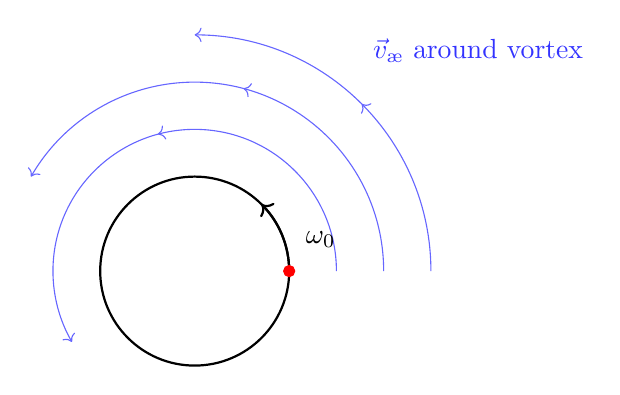
\begin{tikzpicture}[scale=2]
        \usetikzlibrary{decorations.markings}

        % Streamlines with varying arc lengths
        \draw[blue!60, ->,
            postaction={decorate},
            decoration={markings,
            mark=at position 0.5 with {\arrow{>}}}
        ] (0.9,0) arc (0:210:0.9); % Short arc

        \draw[blue!60, ->,
            postaction={decorate},
            decoration={markings,
            mark=at position 0.5 with {\arrow{>}}}
        ] (1.2,0) arc (0:150:1.2); % Medium arc

        \draw[blue!60, ->,
            postaction={decorate},
            decoration={markings,
            mark=at position 0.5 with {\arrow{>}}}
        ] (1.5,0) arc (0:90:1.5); % Long arc

        % Vortexring
        \draw[thick] (0,0) circle (0.6);
        \draw[thick, ->] (0:0.6) arc (0:45:0.6);
        \node at (0.8,0.2) {$\omega_0$};
        \filldraw[red] (0.6,0) circle (1pt);

        % Vectorveld label
        \node[blue!80] at (1.8,1.4) {$\vec{v}_{\ae}$ around vortex};

    \end{tikzpicture}
    \caption{Each $2\pi$ rotation of the vortex core = one tick of the internal clock.}
    \label{fig:wervelklok}
\end{figure}

In this model, a \grqq clock\textquotedblright is realized by a microscopic vortex's rotation. To make this concrete, consider a free particle at rest in the æther. Its vortex core spins steadily, dragging nearby æther around. Let $\omega_0$ denote the angular velocity of this core as measured in the æther rest frame (in units of radians per second). By definition, $\omega_0$ is the particle's \emph{proper rotational frequency}, corresponding to its proper time $\tau$.

We can relate $\omega_0$ to the passage of proper time: if the core rotates by $\Delta \theta$ radians in an interval, then the proper time elapsed is
\[
\Delta \tau = \frac{\Delta \theta}{\omega_0} \,.
\]
For example, if we choose $2\pi$ radians of rotation as a \("\)tick\("\) of the clock, then the proper period is $T_0 = 2\pi/\omega_0$. One might imagine $\omega_0$ is set by the particle's internal structure – e.g., a proton's vortex might rotate at some $10^{23}$ rad/s such that $T_0 \sim 10^{-23}$ s for one revolution (this is speculative, but notably, de Broglie in 1924 proposed that every particle of rest mass $m$ has an internal clock of frequency $mc^2/h$~\cite{deBroglie1924-frequency}, on the order of $10^{21}$ Hz for an electron; a vortex model could provide a physical origin for this \emph{Zitterbewegung} frequency as core rotation).

For now, $\omega_0$ is a free parameter representing the clock rate at rest. When the particle is not free or not at rest, its observed rotation rate can change. We define $\omega_{\textrm obs}$ as the angular velocity of the vortex core as observed by a static æther frame observer (i.e., one at rest with respect to the æther) under whatever circumstances (motion or gravity). The ratio $\omega_{\textrm obs}/\omega_0$ will then give the rate of the clock relative to proper time.

In fact, since $\Delta \tau = \Delta \theta / \omega_0$ always holds for the clock itself, and $\Delta t$ (coordinate time) corresponds to $\Delta \theta / \omega_{\textrm obs}$ (the angle rotated in lab frame time), we have:
\begin{equation}
\frac{\Delta \tau}{\Delta t} = \frac{\Delta \theta / \omega_0}{\Delta \theta / \omega_{\textrm obs}} = \frac{\omega_{\textrm obs}}{\omega_0} \,.
\end{equation}

This important relation links the physical slowdown of the vortex's spin $\omega_{\textrm obs}$ to the time-dilation factor. If $\omega_{\textrm obs} < \omega_0$, the clock runs slow (since $\Delta \tau < \Delta t$).

Our task in the next sections is to determine $\omega_{\textrm obs}$ for two cases:
\begin{enumerate}
    \item When the vortex (particle) moves at velocity $v$ through the æther,
    \item When the vortex sits in a gravitational potential (æther flow) created by a massive body.
\end{enumerate}
We will find that $\omega_{\textrm obs}/\omega_0$ in these cases reproduces the familiar Lorentz and gravitational time dilation factors, respectively.

Before we proceed, we emphasize that \emph{proper time $\tau$ in this model is fundamentally just a count of the rotation of the vortex}. This provides an objective, mechanistic picture of time: for example, one could imagine a small flag or marker on the vortex core completing laps around the core—each lap is an unambiguous physical event corresponding to a fixed amount of proper time. Different physical clocks (atoms, molecules, etc.) would all eventually trace their time to such microscopic circulations in the universal æther.

For a discussion of how composite clocks consisting of multiple vortex nodes collectively experience time dilation, see Appendix~ \hyperref[appendix:ClocksInVortexStructures]{A}

As long as the laws of physics are such that these circulations are stable and identical for identical particles, this provides a standard of time. We then show how motion through the æther and æther currents affect $\omega_{\textrm obs}$.
\section{Time Dilation from Relative Motion}

First, consider time dilation for a particle moving at high speed relative to the æther rest frame. Empirically, we know that a clock moving at velocity $v$ experiences time slower by the Lorentz factor $\gamma = 1/\sqrt{1 - v^2/c^2}$. In this model, we derive the same effect by analyzing the influence of absolute æther motion on vortex core rotation.

\subsection*{(a) Kinematic Derivation}

Let a vortex be at rest in its own frame $S'$ but moving at velocity $v$ relative to the æther rest frame $S$. In $S'$, the vortex rotates with angular frequency $\omega_0$, and defines proper time $\tau$. Due to Lorentz time dilation, an observer in $S$ sees the clock slow down:

\begin{figure}[htbp]
    \centering
    \includegraphics[width=0.85\textwidth]{06-TijddilatatieBeweging}
    \caption{Effect of æther flow on the internal rotation velocity of a vortex particle. At rest (left), the vortex retains its maximum angular velocity~$\omega_0$. When moving through the æther (right), the flow causes a reduced observed angular velocity to~$\omega_{\mathrm{obs}} < \omega_0$.}
    \label{fig:TijddilatatieBeweging}
\end{figure}

\[
\omega_\text{obs} = \omega_0 \sqrt{1 - \frac{v^2}{c^2}} \,.
\]
From the relation between proper and coordinate time,
\begin{equation}
\frac{d\tau}{dt} = \frac{\omega_\text{obs}}{\omega_0} = \sqrt{1 - \frac{v^2}{c^2}} \,.
\end{equation}

This matches the standard SR time dilation formula. In our model, the physical mechanism is that æther motion across the vortex disrupts its swirl rate, slowing the apparent rotation in the æther frame.

\subsection*{(b) Fluid-Dynamic Interpretation}

A complementary interpretation uses compressible flow analogies. In fluid dynamics, a body moving at speed $v$ in a compressible medium with signal speed $c$ experiences distortions proportional to $\gamma = 1/\sqrt{1 - v^2/c^2}$. This can be thought of as a Doppler time dilation or resistance to maintaining coherent circulation. 

As velocity approaches the æther signal speed $c$, the surrounding flow compresses and resists vortex rotation. Therefore, the angular velocity seen in the æther frame drops, and:
\begin{equation}
\omega_\text{obs} = \omega_0 \sqrt{1 - \frac{v^2}{c^2}} \Rightarrow \frac{d\tau}{dt} = \sqrt{1 - \frac{v^2}{c^2}} \,.
\end{equation}

In fluid dynamics, the Prandtl–Glauert factor explicitly characterizes compressible flow disturbances around objects moving near a medium's characteristic signal speed $c$. As velocity approaches this speed, fluid disturbances become increasingly resistant to propagation forward, closely analogous to the ætheric reduction of vortex core rotation at high velocities. Thus, the emergence of the Lorentz factor $\gamma$ in our model is physically and mathematically analogous to fluid compressibility effects.

\subsection*{Implication}

This gives us the relativistic time dilation for a moving clock:
\[
\boxed{\frac{d\tau}{dt} = \sqrt{1 - \frac{v^2}{c^2}}}
\]
within a Euclidean, æther-based flat space, and matches all special relativity experimental predictions~\cite{Rado2020-æther-Lorentz,Levy2009-æther-clock}.

\section*{Generalized Dilation from Swirl Field Tension}\label{sec:generalized_dilation}

For non-inertial or vortex-deformed systems (e.g. near a massive vortex), time dilation also includes effects from swirl tension gradients. Let $\gamma(\vec{x})$ be a local swirl factor based on local curvature energy of the vortex core:

\[
\gamma(\vec{x}) = \sqrt{1 - \frac{\Phi(\vec{x})}{\Phi_{\text{max}}}}
\]

where $\Phi$ is the swirl energy density (linked to vortex line tension), and $\Phi_{\text{max}}$ is the limiting swirl energy. Time slows in high-tension regions:

\[
d\tau = \gamma(\vec{x})\, d\mathcal{N}
\]

This formulation unites translational and rotational effects and maps to gravitational redshift:
\[
\text{For weak fields: } \Phi \sim \frac{G M}{r}, \quad \text{For vortex curvature: } \Phi \sim \frac{\Gamma^2}{r^2}
\]

Time dilation here stems from topological distortion of the swirl field—not spacetime curvature.

\section{Gravitational Time Dilation via Æther Flow}

In General Relativity, clocks deeper in a gravitational potential well run slower compared to those at higher potentials. We reproduce this result using æther flow fields instead of spacetime curvature. In the Vortex Æther Model, the effect is expressed as local variations in swirl field energy and æther inflow velocity.

\subsection*{5A. Æther Flow as Gravity}

We assume that mass $M$ induces an inward radial flow of æther. At a radius $r$, this flow speed is given by:
\[
v_g(r) = \sqrt{\frac{2GM}{r}}.
\]

\begin{figure}[htbp]
    \centering
    \includegraphics[width=0.85\textwidth]{images/07-GravitationeleÆtherinstroom}
    \caption{Gravitational time dilation due to radial æther inflow towards a mass~$M$. The vortex clock experiences a lower angular velocity due to æther drag, analogous to the Schwarzschild redshift.}
    \label{fig:GravitationeleÆtherinstroom}
\end{figure}

This mirrors the Painlevé–Gullstrand metric and the river model of black holes~\cite{Hamilton2004-river}.

\subsection*{Æther Drag and Clock Slowdown}

A clock held at radius $r$ in this inward æther flow sees æther moving past it at speed $v_g(r)$. The vortex core's observed angular velocity is therefore reduced due to the æther's drag, just as in the special relativity case, where motion through æther reduces the observed clock rate.

Thus, the gravitational time dilation factor is:
\begin{equation}
\frac{d\tau}{dt} = \sqrt{1 - \frac{v_g^2(r)}{c^2}} = \sqrt{1 - \frac{2GM}{rc^2}}.
\end{equation}

A notable implication of gravitational æther inflow is related to the maximum force principle, defined as $F^{\text{max}}_{\text{gr}} = c^4 /4G$. Physically, this represents the upper limit on æther drag forces, where the inward æther flow near gravitational horizons reaches velocities close to $c$. At the Schwarzschild radius, the inflow speed of æther matches this limit, effectively freezing the rotation of any vortex-based clocks due to extreme drag, thus providing a tangible fluid-mechanical interpretation of gravitational horizons.

This is consistent with the Schwarzschild solution for stationary observers in general relativity.

A precise confirmation of gravitational time dilation under controlled conditions was provided by the Gravity Probe A mission~\cite{vessot_levine_1980}, which launched a hydrogen clock to an altitude of 10,000 km.

This delay was not only derived theoretically, but was confirmed experimentally by Pound and Rebka in 1959, who measured a gravitationally induced frequency shift between two points at different altitudes within the Earth's gravitational field using the Mössbauer effect~\cite{pound_rebka_1959}.

\subsection*{Interpretation}

This equation means that the deeper a vortex is located in the gravitational potential (the faster the local æther flow), the slower it rotates from the perspective of an observer at infinity. At the Schwarzschild radius $r_s = 2GM/c^2$, $d\tau/dt = 0$: time stops for external observers.

This provides a mechanistic interpretation of gravitational redshift: light emitted by a vortex-clock in a strong potential well appears redshifted due to the slower angular motion of the emitting vortex. The result:
\[
\boxed{\frac{d\tau}{dt} = \sqrt{1 - \frac{2GM}{rc^2}}}
\]
is fully consistent with GR and supports the æther flow analogy~\cite{Schiller2022-maxforce}.

\subsection*{5B. Alternative Derivation via Swirl Tension Field}

The same dilation can be derived using the generalized topological swirl field from Section~\ref{sec:generalized_dilation}. Let $\Phi(\vec{x})$ be the swirl energy density due to curvature of vortex cores or gravitational tension. Then the local dilation becomes:

\[
\frac{d\tau}{d\mathcal{N}} = \sqrt{1 - \frac{\Phi(\vec{x})}{\Phi_{\text{max}}}}
\]

This includes both the gravitational case and other scenarios where curvature increases vortex twist or core strain. For gravity, one may take $\Phi \sim GM/r$ or $\Phi \sim \Gamma^2/r^2$. This tension-driven dilation provides a unified formalism for gravitational and relativistic slowdown in VAM.

\subsection*{5C. Bernoulli Interpretation via Æther Pressure Gradients}

A third interpretation uses Bernoulli's law for superfluids. Here, gravitational potential is seen as a reduction in æther pressure near masses. According to Bernoulli's principle, a lower æther pressure corresponds to higher local flow speed and tension. This directly maps to vortex time dilation, and complements the inflow model by associating energy density with pressure drops.

Together, these views frame gravitational dilation as a result of:
\begin{itemize}
    \item Inward æther flow (kinematic drag),
    \item Vortex curvature energy (swirl tension),
    \item Æther pressure drop (fluid potential).
\end{itemize}

This confirms the robustness and physical interpretability of time dilation within the Vortex Æther Model.

\section{Combined Effects and Further Predictions}

Having derived separate time dilation factors for motion through æther and gravitational æther flow, we now consider both effects simultaneously.

\subsection*{Combined Motion and Gravitational Field}

Let a vortex-clock move with velocity $\vec{u}$ in a region where the æther is flowing with velocity $\vec{v}_g$. The effective relative velocity with respect to the local æther flow is:
\[
\vec{v}_\text{rel} = \vec{u} - \vec{v}_g.
\]
The observed time dilation is then:
\[
\frac{d\tau}{dt} = \sqrt{1 - \frac{|\vec{v}_\text{rel}|^2}{c^2}}. \tag{5}
\]
This formulation smoothly incorporates both special and general relativistic effects into a single expression.

\subsection*{Example: Circular Orbit Time Dilation}

Consider a clock orbiting a mass $M$ at radius $r$. The tangential velocity of the orbit is:
\[
v_\text{orb} = \sqrt{\frac{GM}{r}}, \quad v_g(r) = \sqrt{\frac{2GM}{r}}.
\]
Since the orbital velocity is perpendicular to the radial æther inflow, the relative speed is:
\[
v_\text{rel} = \sqrt{v_\text{orb}^2 + v_g^2} = \sqrt{\frac{3GM}{r}}.
\]

\begin{figure}[htbp]
    \centering
    \includegraphics[width=0.85\textwidth]{08-BaanRondMassa}
    \caption{A vortex in a circular orbit experiences combined time dilation due to orbital and æther flow. The clock experiences both orbital velocity~$\vec{v}_{\mathrm{orb}}$ and æther inflow~$\vec{v}_g$, which together result in a combined relative velocity~$\vec{v}_{\mathrm{rel}}$.}
    \label{fig:BaanRondMassa}
\end{figure}

Thus, the time dilation becomes:
\[
\frac{d\tau}{dt} = \sqrt{1 - \frac{3GM}{rc^2}}. \tag{6}
\]
This matches the exact result from Schwarzschild geometry for circular orbits.

\begin{figure}[htbp]
    \centering
    \includegraphics[width=0.85\textwidth]{09-CombinedTimeDilationSurface}
    \caption{Visual representation of the time dilation factor \( \frac{d\tau}{dt} \) as a function of both the orbital velocity \( v_\text{orb} \) and the gravitational æther inflow velocity \( v_g \). The surface shows how both contributions — inertial and gravitationally derived æther flow — together result in a total slowing down of the clock. The hyperbolic curvature of the surface reflects the combined Lorentz and Schwarzschild dilation as described in equations (5) and (6).}
    \label{fig:TimeDialationCombined}
\end{figure}

\subsection*{Implications Near a Horizon}

As $r \to r_s = 2GM/c^2$, the inflow speed $v_g(r)$ approaches $c$, and any static observer's clock slows to zero. The æther flow fully suppresses local vortex rotation, providing a natural mechanism for the \("\)freezing of time\("\) at the event horizon.

\begin{figure}[htbp]
    \centering
    \includegraphics[width=0.85\textwidth]{10-HorizonTijdsbevriezing}
    \caption{Æther flow accelerates towards $r_s$, where the observed clock rotation becomes zero. Freezing of time at the event horizon $r = r_s$: the Æther flow approaches~$c$, causing $\omega_{\mathrm{obs}} \to 0$. On the right, the corresponding decrease in $\frac{d\tau}{dt}$ as a function of distance is shown.}
    \label{fig:HorizonTijdsbevriezing}
\end{figure}


\subsection*{Quantum and Cosmic-Scale Consistency}

This vortex-æther framework naturally explains relativistic phenomena consistently across scales—from quantum to cosmic. For instance, at quantum scales, the observed lifetime dilation of rapidly moving muons directly results from reduced internal vortex rotation frequency in relativistic æther flows. At cosmic scales, near black hole horizons, vortex rotation essentially freezes due to æther inflow approaching ccc, providing a concrete physical mechanism for horizon phenomena. Such scale invariance underscores the comprehensive explanatory power of the æther model.

\subsection*{Unified Interpretation}

\begin{figure}[htbp]
    \centering
    \includegraphics[width=0.85\textwidth]{11-TijdsvertragingRelatieveBeweging}
    \caption{Universal time dilation formula in the Vortex Æther Model. The clock rate decreases with increasing relative velocity~$|\vec{v}_{\mathrm{rel}}|$ with respect to the æther. At $|\vec{v}_{\mathrm{rel}}| = c$ time stops.}
    \label{fig:TijdsvertragingRelatieveBeweging}
\end{figure}

This æther model allows all relativistic time dilation effects to be viewed as consequences of one principle:
\[
\text{Clock rate reduction} \;\propto\; \text{relative motion through æther}.
\]
Whether this relative motion arises from inertial velocity or from ætheric inflow due to nearby mass, the observable consequence is the same. Therefore, we conclude:
\[
\boxed{\frac{d\tau}{dt} = \sqrt{1 - \frac{|\vec{u} - \vec{v}_g|^2}{c^2}}}
\]
as the general time dilation formula for the Vortex Æther Model.
For possible experimental deviations of these time dilation formulas from general relativity, see Appendix-B~\ref{appendix:DeviatingPredictions}.

\section{Conclusion}

We have derived time dilation laws within a 3D Euclidean æther model, where particles are modeled as vortex knots, and time is defined by their intrinsic vortex core rotation. Motion through the æther and ætheric inflows (gravitational fields) reduce the observable angular velocity of vortex rotation, yielding:

\begin{itemize}
    \item The special-relativistic time dilation:
    \[
    \frac{d\tau}{dt} = \sqrt{1 - \frac{v^2}{c^2}},
    \]
    which arises from absolute motion through the æther.
    
    \item The gravitational time dilation:
    \[
    \frac{d\tau}{dt} = \sqrt{1 - \frac{2GM}{rc^2}},
    \]
    which arises from inward æther flow near mass $M$.
    
    \item The unified general case:
    \[
    \frac{d\tau}{dt} = \sqrt{1 - \frac{|\vec{u} - \vec{v}_g|^2}{c^2}},
    \]
    covering motion in a gravitational field.
\end{itemize}

These results accurately reproduce predictions of special and general relativity using physically intuitive mechanisms grounded in fluid dynamics.

The æther model eliminates the need for curved spacetime by replacing it with structured velocity fields in flat space. It reinterprets relativistic time effects as real, mechanical consequences of vortex core dynamics interacting with a physical æther.

This approach couples microphysics (vortex core rotation) with cosmological structure (black hole horizons) and maintains continuity across scales. By interpreting time dilation as angular deceleration of vortices, this model provides a mechanistic, field-based alternative to geometric spacetime curvature, preserving experimental consistency with SR and GR while opening possibilities for fluid dynamical extensions of fundamental physics~\cite{Winterberg2002-PlanckÆther,Schiller2022-maxforce}.

Future work may include deriving Einstein's field equations of conservation of æther vorticity or testing laboratory analogues via superfluid experiments. The reinterpretation of black hole horizons, gravitational redshift, and quantum timekeeping via vortex rotation encourages deeper theoretical and experimental investigations into the role of æther in modern physics.

A more extensive elaboration of these ideas can be found in the follow-up study: \textit{\grqq Swirl Clocks and Vorticity-Induced Gravity\textquotedblright } (2025).~\cite{vam2025unified}.

\appendix \label{sec:Part-6}
\section*{Appendix A: Macroscopische Klokken als Samengestelde Wervelstructuren}
\label{appendix:KlokkenInWervelstructuren}

In het Vortex Æther Model (VAM) wordt tijd gedefinieerd als de interne rotatie van een wervelkern. Dit roept de vraag op hoe macroscopische klokken, zoals atoomklokken of fotonenoscillatoren, tijddilatatie ondervinden wanneer zij bestaan uit een ensemble van wervelknopen.

\subsection*{Tijddilatatie van individuele wervels}

Volgens het model ondergaat een enkele wervelknoop tijddilatatie gegeven door:
\begin{equation}
    d\tau = \frac{1}{\Omega} \, d\theta = dt \cdot \sqrt{1 - \frac{v_\text{rel}^2}{c^2}} \label{eq:single_tau}
\end{equation}
waarbij \( \Omega \) de intrinsieke hoeksnelheid is van de wervelkern, en \( v_\text{rel} \) de relatieve snelheid van de wervel ten opzichte van de lokale ætherstroom.

\subsection*{Samengestelde wervelsystemen}

Beschouw een macroscopisch systeem met \( N \) wervelknopen, elk met lokale hoeksnelheid \( \Omega_i \). De effectieve tijdstoename voor het totale systeem is:
\begin{equation}
    \langle d\tau \rangle = \frac{1}{N} \sum_{i=1}^{N} \frac{1}{\Omega_i} \, d\theta_i \label{eq:ensemble}
\end{equation}

Wanneer het systeem coherent is — bijvoorbeeld in een kristal of atoomklok — dan geldt \( \Omega_i \approx \Omega \), en dus:
\begin{equation}
    \langle d\tau \rangle \approx \frac{1}{\Omega} \, d\theta \tag{\ref{eq:ensemble}'}
\end{equation}
wat gelijk is aan de tijddilatatie van een enkelvoudige wervel (vergelijking~\ref{eq:single_tau}).

\subsection*{Decoherente systemen}

Bij decoherente of chaotische systemen variëren de relatieve snelheden \( v_{\text{rel}, i} \) per wervel. Dan geldt:
\begin{equation}
    \langle d\tau \rangle = \left\langle \sqrt{1 - \frac{v_{\text{rel}, i}^2}{c^2}} \right\rangle dt
\end{equation}
Wat in eerste orde benaderd wordt als:
\begin{equation}
    \langle d\tau \rangle \approx dt \cdot \sqrt{1 - \frac{\langle v_\text{rel}^2 \rangle}{c^2}} \label{eq:average_dil}
\end{equation}

\subsection*{Conclusie}

Zowel in coherente als in decoherente systemen is de totale tijddilatatie consistent met de individuele dilatatie van de onderliggende wervelknopen. Dit verklaart waarom complexe systemen — atoomklokken, kristallen, biologische ritmes — universeel vertraagd lopen in zwaartekrachtvelden of bij hoge snelheden: hun interne structuur is opgebouwd uit dezelfde roterende vorticiteitskernen.

\vspace{1em}
\noindent
Deze afleiding bevestigt dat het VAM-model schaalonafhankelijk functioneert en tijddilatatie reproduceert op zowel micro- als macroscopisch niveau.
\section*{Appendix B: Afwijkende Voorspellingen ten opzichte van Algemene Relativiteit}

Het Vortex Æther Model (VAM) reproduceert veel bekende resultaten van de algemene relativiteit (GR), maar suggereert ook een aantal experimenteel toetsbare afwijkingen in regimes waar de klassieke geometrische theorie geen expliciete verklaring biedt. Hieronder formuleren wij drie concrete situaties waarin het VAM-model predicties maakt die (in principe) afwijken van GR.

\subsection*{1. Tijdsdilatatie in roterende superfluïda}

In roterende superfluïden zoals vloeibaar helium of Bose-Einstein Condensaten (BECs), ontstaan macroscopische kwantumvortices met meetbare angular velocity \( \omega \). Binnen VAM geldt lokale tijdsdilatatie via:

\begin{equation}
    d\tau = dt \cdot \sqrt{1 - \frac{\omega^2 R^2}{c^2}},
\end{equation}

waarbij \( R \) de afstand tot het wervelcentrum is. Dit effect is meetbaar via klokverschuivingen op µs-schaal indien men atoomklokken plaatst op verschillende locaties binnen een roterende BEC.

\subsection*{2. Vorticiteitsafhankelijke vertraging in LENR-achtige systemen}

VAM voorspelt dat bij sterk oscillatoire elektromagnetische cavitatie (zoals bij laagenergetische kernreacties) een lokale swirl-potentiaal ontstaat:

\begin{equation}
    \Phi_{\text{swirl}} = \frac{1}{2} \omega^2 r^2 \Rightarrow \Delta \tau \sim \frac{\Phi_{\text{swirl}}}{c^2} \cdot dt.
\end{equation}

Hierdoor zou interne tijd in wervelrijke nano-structuren meetbaar vertragen. Toepassing op Pd/D-elektroden met µs-resolutie kan deze vertraging detecteren via optische meetintervallen of anomalieën in gamma-ruisprofielen.

\subsection*{3. Lichtafbuiging zonder ruimtetijdkromming}

In plaats van geodetische afbuiging in een gekromde ruimte, beschouwt VAM licht als stromend in een æther met inhomogene snelheid. De afbuiging volgt dan uit een brekingsgradiënt:

\begin{equation}
    \nabla n(\vec{r}) = \frac{1}{c} \frac{\partial v_\ae}{\partial r} \Rightarrow \delta \theta = \int \frac{dn}{dr} \, dr,
\end{equation}

wat experimenteel testbaar is via analoge zwaartekrachtsimulaties in roterende vloeistofbakken of optische metamaterialen met swirl-indexverloop.

\bigskip

Deze scenario’s tonen aan dat het VAM-model experimenteel onderscheidend gedrag voorspelt in situaties waar GR neutraal of onvoorspellend is. Verdere experimentele validatie is noodzakelijk om de toepasbaarheid van deze voorspellingen vast te stellen.

        \bibliographystyle{unsrt}
        \bibliography{../references}
\end{document}